\documentclass{article}

\usepackage[utf8]{inputenc}
\usepackage{graphicx}
\usepackage{caption}
\usepackage{subcaption}

\begin{document}

\section*{Introduction}
For this practical session, we use Kmeans to cluster data based on their locations to find all attractive regions.
%
We use python to process our data, train our model and predict.
%
Our data set came from Flick which is a Yahoo photo sharing system and consists of locations, upload time, user id and description, etc.. 
%
But we just used locations we wanted to find attractive regions.
%
We found that we have to set the size of different clusterings to find the clearest results.

\par

At first we got our results and just plotted it without map. We just wanted to make sure it works.
%
The first time we converted many columns to one colum "date upload time" and used category to represent it.
%
And we trained based on location, user id, picture id and upload time.  
%
The point cloud we got was really fuzzy, there was no cluster actually.
%
Finally, we found that that was because we used so many non relevant columns.
%
After we dropped some other columns except locations, it was very clear.
%
We could get something explicitly through out plotting.

\par
After we finished this, we added our map as background.
%
And we grouped them based on the same predict result and ploted group by group.
%
We found that tete park and bellecour were really attractive.
 
\section*{Implementation}
\par
We decided to just implement clustering in Python without KNIME. Immediately we ran into issues with the size of the the initial dataset.
When looking at the .csv file in the PyCharm IDE, the whole IDE would freeze. After realizing that this was our problem and not Pythons processing 
ability, we moved on. Our first step was to build date taken and date upload from the current columns in the dataset. Since it was not well 
represented initial, this was to be done first. After our new columns replaced the old ones we still had too many columns. As pointed out 
by someone in our class, there were a lot of repeated columns. This was easy to add in and made our dataset go from 167702 
data points to just 13504. 
\par 
Now we can implement clustering. We started out using the K-Means clustering algorithm. Once we ran the code, we waited and waited and waited.
Clearing there was too many iterations and too much data to be processed. We tried minimizing the data as much as possible however, nothing
was fixing the computation time. Luckily, there was MiniBatchKMeans which splits the dataset into small batches for faster computation. 
Based on the sckit API was was little to no different between the two implementations. After we were able to let the 
clustering algorithm run efficiently, we then plotted our data. We started off our clustering by using the latitude, longitute, and upload date and time. 
However, this gave us some weird results on our graph. The clusters were very undefined and it seemed like it wasn't working. Then it was
clear that including the upload and taken dates were causing the undefined clusters. We removed them from the computation of the clustering, and 
we just used latitude and longitute. This resulted in much clearer results. We could see clear separations of our data. But at this point, 
we were plotting the values to a blank plot. But these were coordinates on a map, so we took a picture of a map that was defined by our coordinates
and used it as the background to our scatter plot. This was not the best solution but it was good enough for us to interpret the data as a location. 
Once we had completed our program, we then created multiple graphs using different sized clusters for analysis. 


\section*{Results}
Explain our results!

\begin{figure}[!h]
  \centering
  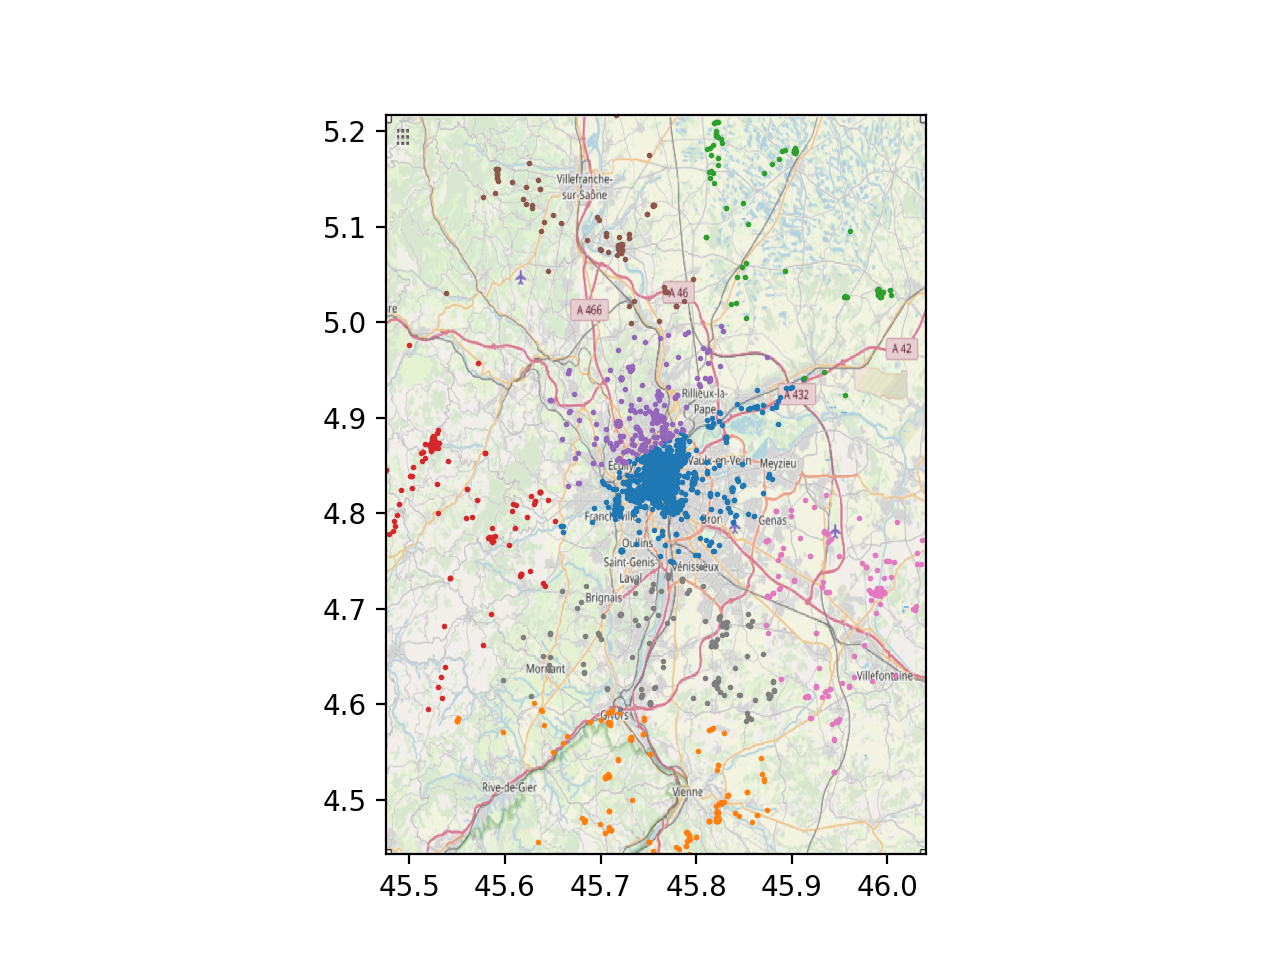
\includegraphics[width=0.5\textwidth]{small_clusters_8.png}
  \caption{clusters size is 8}
  \label{fig:clusters_8}
\end{figure}


\begin{figure}[!h]
  \centering
  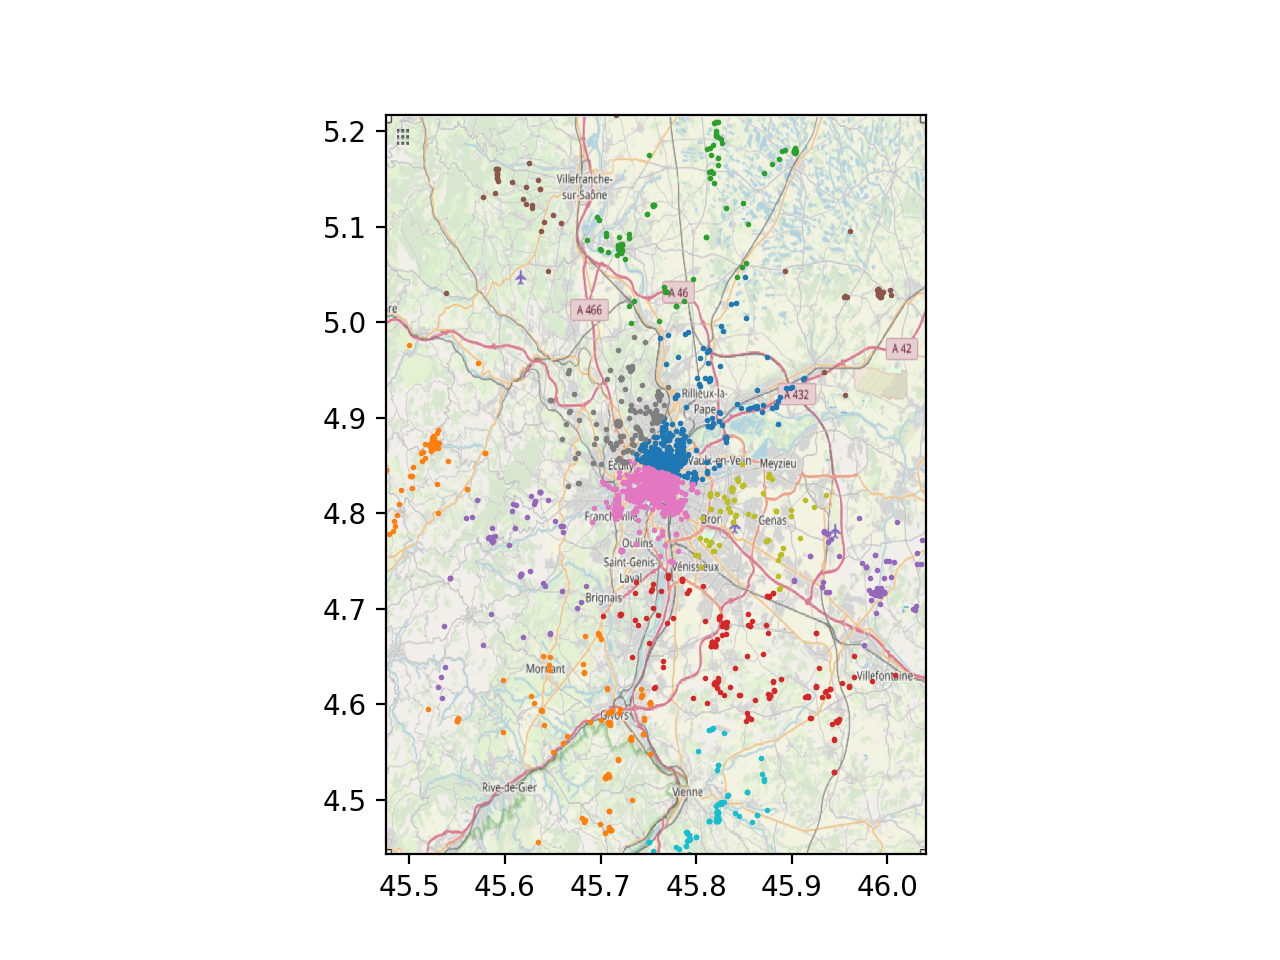
\includegraphics[width=0.5\textwidth]{medium_clusters_16.png}
  \caption{clusters size is 16}
	\label{fig:clusters_16}
\end{figure}

\begin{figure}[!h]
  \centering
  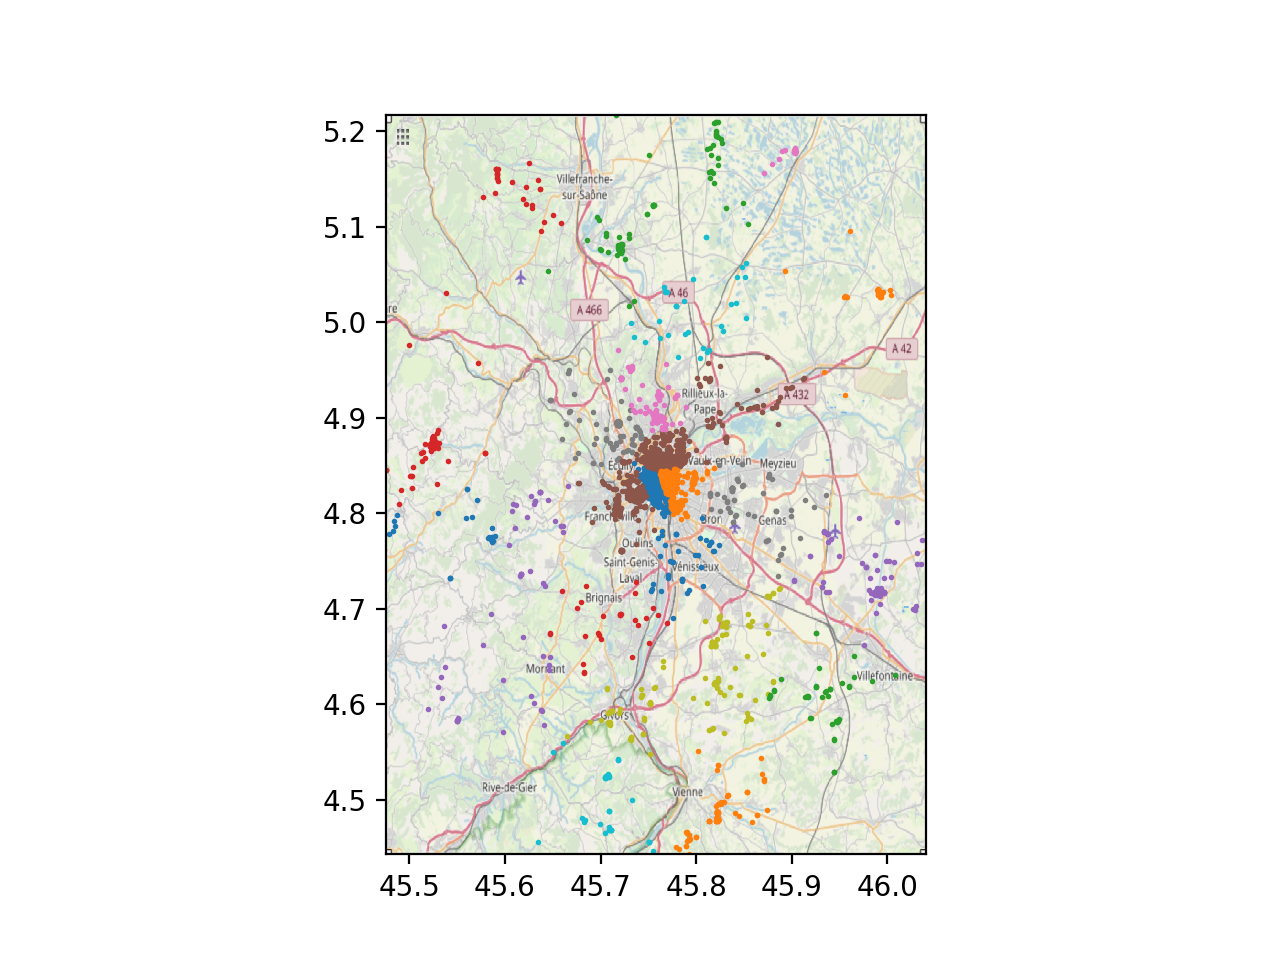
\includegraphics[width=0.5\textwidth]{clustering_26_full.png}
  \caption{clusters size is 26 full}
	\label{fig:clusters_26_full}
\end{figure}

\begin{figure}[!h]
  \centering
  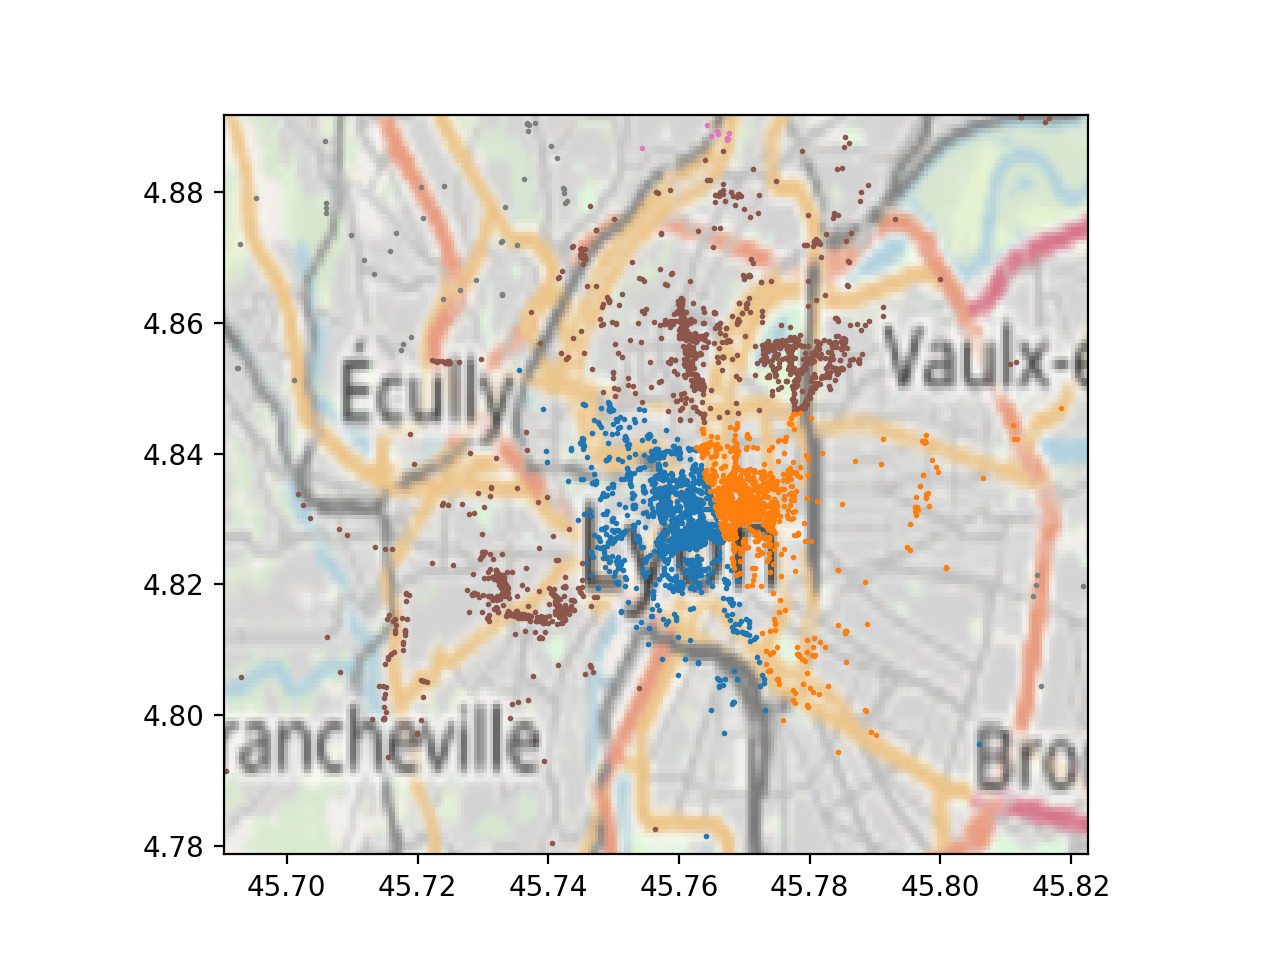
\includegraphics[width=0.5\textwidth]{clustering_26_zoomed.png}
  \caption{clusters size is 26 and zoomed}
	\label{fig:clusters_26_zoomed}
\end{figure}

\begin{figure}[!h]
  \centering
  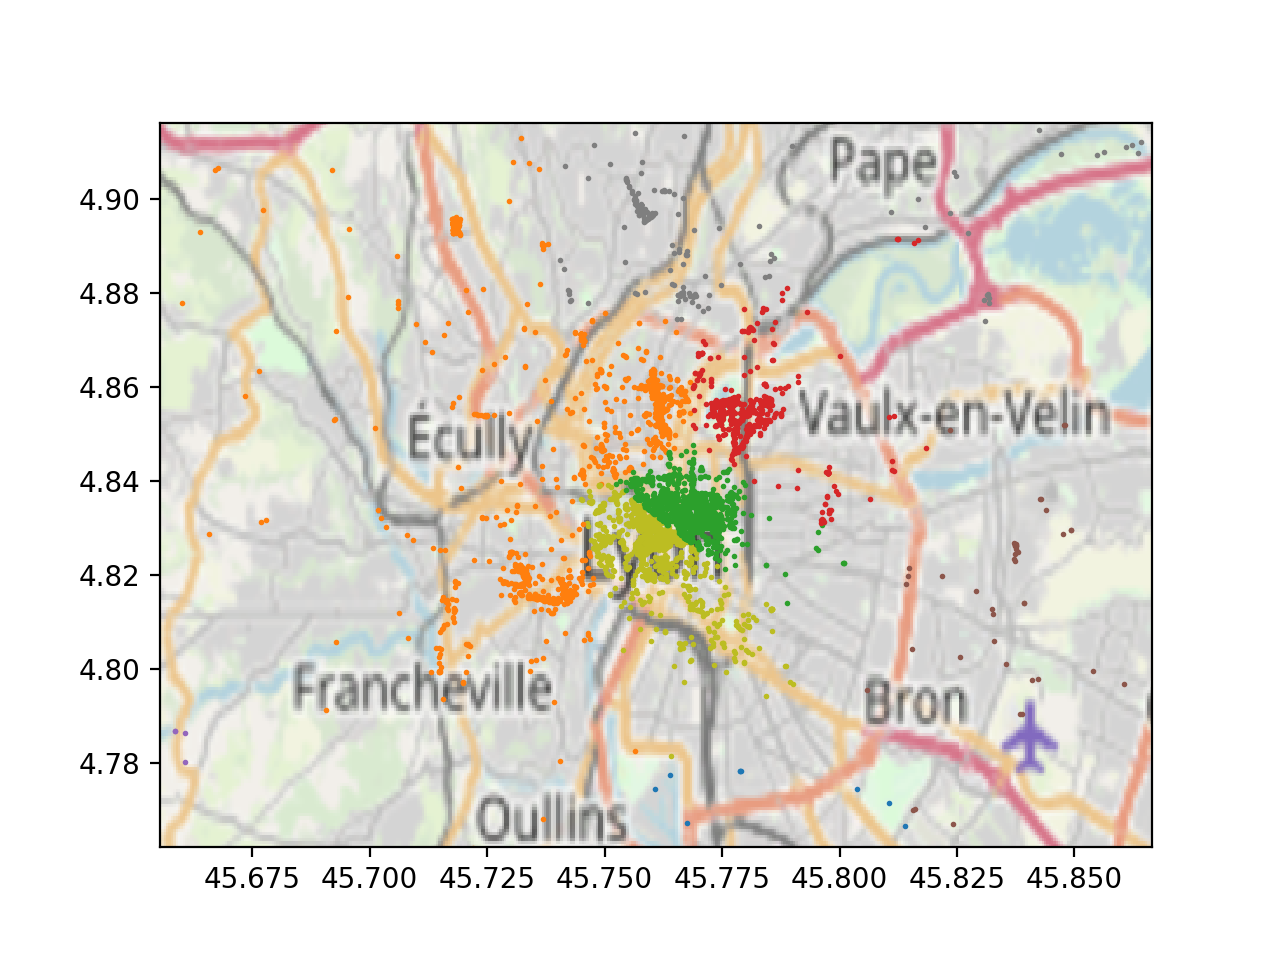
\includegraphics[width=0.5\textwidth]{clustering_32_zoomed.png}
  \caption{clusters size is 32 and zoomed}
	\label{fig:clusters_32_zoomed}
\end{figure}

\begin{figure}[!h]
  \centering
  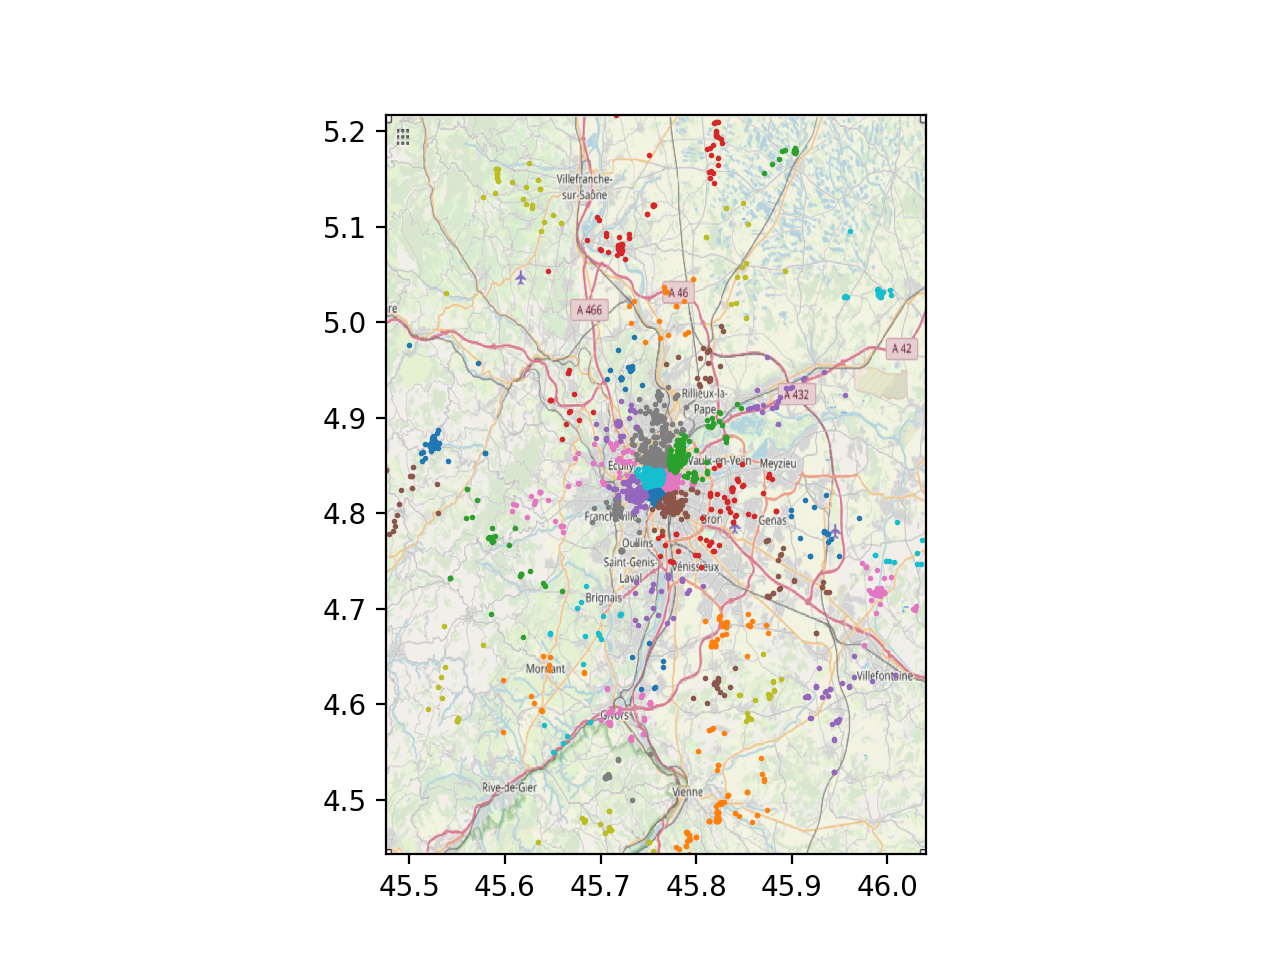
\includegraphics[width=0.5\textwidth]{clustering_50.png}
  \caption{clusters size is 50}
	\label{fig:clusters_50}
\end{figure}








\end{document}
